\documentclass[a4paper,twoside,openany,12pt]{memoir}

% Memoir linespacing
\DoubleSpacing

% LaTeX packages
\usepackage{amsmath}
\usepackage{amsfonts}
\usepackage{amssymb}
\usepackage{bigfoot}
\usepackage{bm}
\usepackage{caption}
\usepackage{color}
\usepackage{graphicx}
\usepackage{indentfirst}
\usepackage[utf8]{inputenc}
\usepackage[
  safeinputenc,
  style=phys,
  backend=biber,
  sorting=none,
  minnames=10,
  maxnames=10,
  biblabel=brackets
]{biblatex}
\addbibresource{references.bib}
\usepackage{libertine}
\usepackage{lipsum}
\usepackage{oxfordthesis}
\usepackage{xr}
\usepackage{xr-hyper}

% Title / Author / Date / Degree / etc.
\thetitle{Thesis title}
\theauthor{Ferdinand van Wyk}
\degreedate{Jan 2017}
\degree{Doctor of Philosophy}
\college{Mansfield College}
\university{University of Oxford}


\usepackage[
	pdftitle={\oxfthetitle},
	pdfauthor={\oxftheauthor},
	pdfsubject={Thesis for the Degree of \oxfdegree, \oxfdegreedate},
	pdfborder=0,
	bookmarks=true,
	bookmarksnumbered=true,
	bookmarksopen=true,
	bookmarksopenlevel=1,
	plainpages=false,
	pdfpagelabels=true,
	colorlinks=false,
    citecolor=blue
]{hyperref}
\usepackage{memhfixc}

% Your Macros File Here
% Useful macros
\newcommand{\figref}[1]{Figure~\ref{fig:#1}}
\newcommand{\figsref}[2]{Figures~\ref{fig:#1} and~\ref{fig:#2}}
\newcommand{\figsdash}[2]{Figures~\ref{fig:#1} -- \ref{fig:#2}}
\newcommand{\Figref}[1]{Figure~\ref{fig:#1}}
\newcommand{\Figsref}[2]{Figures~\ref{fig:#1} and~\ref{fig:#2}}
\newcommand{\Figsdash}[2]{Figures~\ref{fig:#1} -- \ref{fig:#2}}
\newcommand{\Secref}[1]{Section~\ref{#1}}


% Main document

\begin{document}

\titlepage

\frontmatter

\begin{dedication}
Dedicated to whomever
\end{dedication}

\begin{acknowledgements}
  \lipsum[1]
\end{acknowledgements}

\begin{abstract}
  \lipsum[1-2]
\end{abstract}









\tableofcontents
\listoffigures

\mainmatter

\chapter{Introduction}

Here are some references~\cite{Highcock2012, Abel2013, VanWyk2016} and
\figref{torus}, followed by some text.

\begin{figure}[t]
  \centering
  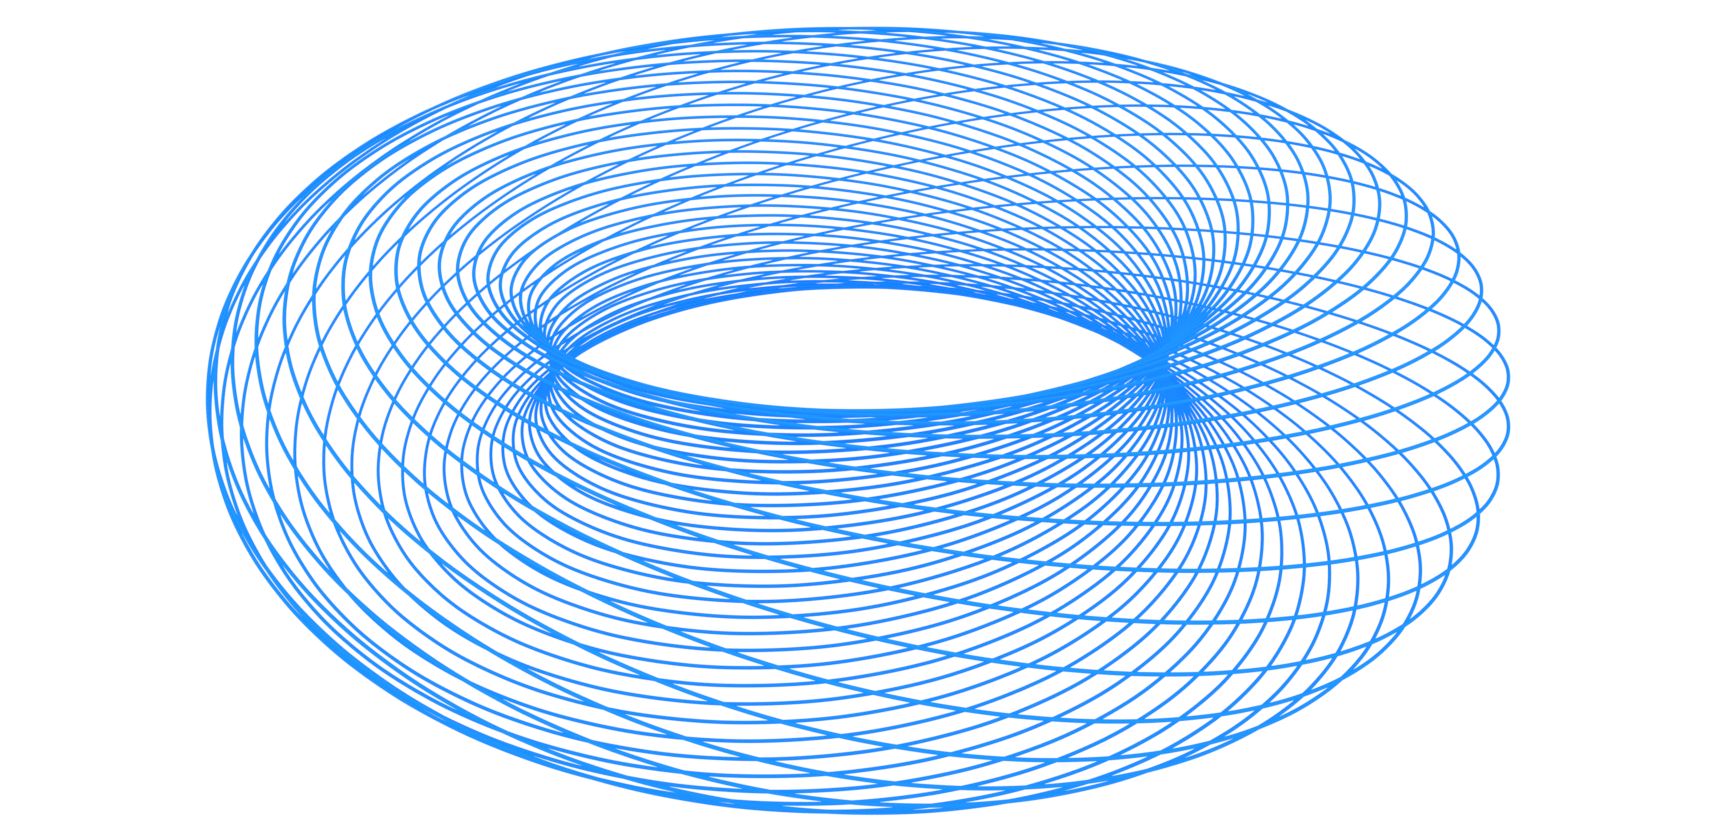
\includegraphics[width=0.7\linewidth]{figures/torus.png}
  \caption[Figure title]{Caption text}
  \label{fig:torus}
\end{figure}

\lipsum[1-3]

\chapter{Chapter title}

\lipsum[1-4]

\chapter{Conclusions}

\lipsum[1-4]

\newpage
\appendix

\chapter{Appendix title}

\lipsum[1-4]


\backmatter

\printbibliography

\end{document}
